%%%%%%%%%%%%%%%%%%%%%%%%%%%%%%%%%%%%%%%%%%%%%%%%%%%%%%%

%% Bachelor's & Master's Thesis Template             %%
%% Copyleft by Artur M. Brodzki & Piotr Woźniak      %%
%% Faculty of Electronics and Information Technology %%
%% Warsaw University of Technology, 2019-2020        %%
%%%%%%%%%%%%%%%%%%%%%%%%%%%%%%%%%%%%%%%%%%%%%%%%%%%%%%%

\documentclass[
    left=2.5cm,         % Sadly, generic margin parameter
    right=2.5cm,        % doesnt't work, as it is
    top=2.5cm,          % superseded by more specific
    bottom=3cm,         % left...bottom parameters.
    bindingoffset=6mm,  % Optional binding offset.
    nohyphenation=false % You may turn off hyphenation, if don't like.
]{ee/ee-thesis}

\usepackage[backend=biber]{biblatex}
\usepackage{caption}

\langpol % Dla języka angielskiego mamy \langeng
\graphicspath{{img/}}             % Katalog z obrazkami.
\addbibresource{bibliografia.bib} % Plik .bib z bibliografią

\begin{document}

%--------------------------------------
% Strona tytułowa
%--------------------------------------
\MasterThesis % Dla pracy inżynierskiej mamy \EngineerThesis
\instytut{Elektrotechniki Teoretycznej i Systemów Informacyjno-Pomiarowych}
\kierunek{Informatyka stosowana}
\specjalnosc{Informatyka w Biznesie}
\title{
    Eksperymenty z systemami wieloagentowymi do tworzenia aplikacji biznesowych
}
\engtitle{ % Tytuł po angielsku do angielskiego streszczenia
    Experiments with multi-agent systems for creating business applications
}
\author{inż Konrad Wenc}
\album{330586}
\promotor{dr hab. inż. Bartosz Sawicki}
\date{\the\year}
\maketitle

%--------------------------------------
% Streszczenie po polsku
%--------------------------------------
\cleardoublepage
\streszczenie
Rozwój oprogramowania staje się coraz bardziej złożony, co prowadzi do poszukiwania nowych narzędzi i technologii wspomagających pracę programistów. W ostatnich latach sztuczna inteligencja (AI) zyskała na znaczeniu w różnych aspektach tworzenia oprogramowania, oferując narzędzia automatyzujące zadania, zwiększające efektywność oraz poprawiające jakość kodu. Celem tej pracy jest zbadanie roli agentów AI w procesie tworzenia oprogramowania poprzez przeprowadzenie serii eksperymentów mających na celu ocenę ich użyteczności, wydajności oraz wpływu na jakość oprogramowania.

Praca rozpoczyna się od przeglądu literatury, który prezentuje aktualny stan wiedzy na temat zastosowania AI w rozwoju oprogramowania. Następnie przedstawiono metodologię badań, obejmującą projekt eksperymentu, wybór narzędzi oraz sposób zbierania i analizy danych. W ramach eksperymentów zbadano wydajność wybranych agentów AI w kontekście różnych zadań programistycznych, takich jak generowanie kodu, refaktoryzacja, testowanie i debugowanie.

Wyniki eksperymentów pokazują, że agenty AI mogą znacząco wspomagać programistów w codziennych zadaniach, szczególnie w obszarach automatyzacji i optymalizacji. Jednakże praca ujawnia także pewne ograniczenia technologii AI, w tym wyzwania związane z dokładnością generowanego kodu i jego integracją z istniejącymi systemami. Na podstawie tych wyników przeprowadzono analizę porównawczą tradycyjnych metod programowania z metodami wspomaganymi przez AI.
\slowakluczowe LLM, agent, rozwój oprogramowania

%--------------------------------------
% Streszczenie po angielsku
%--------------------------------------
\newpage
\abstract
Software development is becoming increasingly complex, which leads to the search for new tools and technologies to support the work of programmers. In recent years, artificial intelligence (AI) has gained importance in various aspects of software development, offering tools that automate tasks, increase efficiency, and improve code quality. The aim of this work is to investigate the role of AI agents in the software development process by conducting a series of experiments to assess their usability, performance, and impact on software quality.

The work begins with a literature review that presents the current state of knowledge on the use of AI in software development. Then, the research methodology is presented, including the experimental design, tool selection, and data collection and analysis method. The experiments examine the performance of selected AI agents in the context of various programming tasks, such as code generation, refactoring, testing, and debugging.

The results of the experiments show that AI agents can significantly support programmers in their daily tasks, especially in the areas of automation and optimization. However, the work also reveals some limitations of AI technologies, including challenges related to the accuracy of the generated code and its integration with existing systems. Based on these results, a comparative analysis was conducted between traditional programming methods and AI-assisted methods.
\keywords LLM, agent, software development

%--------------------------------------
% Oświadczenie o autorstwie
%--------------------------------------
\cleardoublepage
\pagestyle{plain}
\makeauthorship

%--------------------------------------
% Spis treści
%--------------------------------------
\cleardoublepage
\setcounter{tocdepth}{2}
\tableofcontents

%--------------------------------------
% Rozdziały
%--------------------------------------
\cleardoublepage
\pagestyle{headings}

\newpage
\section{Wstęp i cel pracy}
Współczesny rozwój oprogramowania staje się coraz bardziej skomplikowany, a presja na szybkie dostarczanie wysokiej jakości produktów wymaga od programistów zarówno dużego nakładu pracy, jak i stosowania narzędzi zwiększających efektywność. W ostatnich latach firmy takie jak OpenAI, Anthropic czy Meta udostępniły duże modele językowe (Large Language Models, LLM), a wraz z nimi powstały narzędzia i biblioteki (zarówno komercyjne, jak i otwarte), umożliwiające budowę systemów wspierających proces wytwarzania oprogramowania.

Obecne badania nad modelami językowymi w kontekście rozwoju oprogramowania, takie jak SWE-bench, przedstawiają test porównawczy dla generowania kodu na podstawie języka naturalnego dla różnych modeli i narzędzi. Wykazano, że modele językowe potrafią generować kod imitujący rzeczywiste poprawki błędów w rzeczywistych repozytoriach, jednak nawet najnowsze modele wykazały tylko 67,6\% skuteczności dla wszystkich badanych problemów \cite{jimenez2024swebenchlanguagemodelsresolve}. Istnieją również bardziej wymagające rankingi ocen jak LiveCodeBench, które badają nie tylko samą generację, lecz również umiejętności naprawy i testowania kodu \cite{jain2024livecodebench}. W obszarze produktywności dużą uwagę przyciągnęły badania nad GitHub Copilot, które w kontrolowanych eksperymentach skróciły czas realizacji zadań o ponad 50\% \cite{peng2023impact}.

W kontekście rozwoju oprogramowania pojawiły się systemy agentowe, takie jak SWE-agent, które dzięki dedykowanemu interfejsowi (Agent-Computer Interface) znacząco poprawiły wyniki na SWE-bench \cite{yang2024sweagent}. Inny nurt rozwoju stanowi MetaGPT, czyli podejście wieloagentowe z rolami i procedurami (SOP), które ogranicza błędy kompozycji i weryfikuje pośrednie wyniki \cite{hong2023metagpt}.

Mimo tych osiągnięć, badania nadal wskazują na brak kompleksowych analiz wpływu agentów AI na cały cykl rozwoju oprogramowania w projektach biznesowych, w tym na jakość, koszt budowy i utrzymywania \cite{cao2025buildbenchmarkrevisiting274}. Dotychczasowe prace koncentrują się głównie na benchmarkach akademickich, eksperymentach w środowisku laboratoryjnym lub wąskich analizach produktywności. Brakuje badań empirycznych w kontekście rzeczywistych projektów biznesowych, gdzie poza czasem realizacji istotne są również takie aspekty jak wskaźnik wad, czytelność kodu czy koszty utrzymania.

\subsection{Cel pracy}
Celem niniejszej pracy jest empiryczna ocena wpływu agentów AI opartych na LLM na proces tworzenia oprogramowania w realistycznym projekcie biznesowym. W szczególności porównanie różnych trybów pracy: tradycyjnego, wspieranego przez pojedyncze LLM oraz opartego o systemy wieloagentowe.

W pomiarach uwzględniono wszechstronne metryki - nie tylko produktywności (czas wykonania), ale także jakości kodu i łatwości w utrzymaniu (złożoność, czytelność) oraz kosztu obliczeniowego (liczba tokenów, czas obliczeń). Weryfikacja wpływu architektury interakcji - sprawdzenie, czy wprowadzenie elementów inspirowanych interfejsem akcji (ACI) oraz procedurami SOP wpływa na efektywność agentów, zgodnie z wynikami raportowanymi w literaturze \cite{yang2024sweagent}.

\subsection{Zakres i struktura pracy}
Praca składa się z kilku zasadniczych części. Pierwsza z nich to przegląd literatury, omówienie aspektów działania modeli językowych, agentów AI oraz ewolucji benchmarków dla LLM (HumanEval, LiveCodeBench), oceny narzędzi wspierających programistów (Copilot), architektur agentowych (SWE-agent, MetaGPT) oraz aktualnych luk badawczych. Następnie przedstawiono użyte narzędzia. Opisano zaprojektowane aplikacje biznesowe oraz dwa warianty podejścia: z pojedynczym agentem i systemem wieloagentowym z elementami ACI/SOP. Metodologia badań – definicja zadań (implementacja, poprawa defektów), metryk (czas, jakość, utrzymywalność, koszt). Zaprezentowano wyniki oraz porównano je do wyników znanych z badań akademickich. Na koniec dokonano interpretacji wyników w kontekście praktycznym oraz omówiono ograniczenia.
\newpage
\section{Wprowadzenie do modeli językowych i systemów agentowych}
Duże modele językowe (ang. \textit{Large Language Models}, w skrócie LLM) stanowią jeden z ważniejszych przełomów w sztucznej inteligencji i dziedzinie przetwarzania języka naturalnego. Potwierdza to fakt, że praca badawcza „Attention is All You Need" \cite{vaswani2023attentionneed} jest jedną z najczęściej cytowanych prac XXI wieku \cite{wikipediaAttentionNeed}. W swojej istocie modele te, oparte na architekturze Transformer, są zaawansowanymi systemami rozpoznawania wzorców w ogromnych zbiorach tekstu. Dzięki mechanizmowi uwagi efektywnie analizują zależności między różnymi częściami tekstu, co prowadzi do lepszego rozumienia języka i kontekstu, a w konsekwencji umożliwia przewidywanie kolejnych słów w sekwencji.

Współczesne modele językowe dzięki nauczaniu maszynowemu na danych pochodzących z różnych dziedzin nauki i dyscyplin, pozwalają na uzyskiwanie odpowiedzi na temat różnych dyscyplin. Wszechstronność LLM-ów doprowadziła do ich przyjęcia w wielu dziedzinach nauki. Doskonale sprawdzają się w tworzeniu treści i pomocy w pisaniu. W rozwoju oprogramowania jako narzędzia do generowania kodu i debugowania stają się coraz popularniejsze, często wyłapując subtelne błędy, które ludzie mogliby przeoczyć. Ich zdolność do rozumienia i analizowania tekstu sprawia, że są potężnymi narzędziami do pomocy w badaniach i analizie danych, podczas gdy ich zdolności rozumienia języka umożliwiają wykonywanie takich zadań jak tłumaczenia i podsumowania, po bardziej zaawansowane jak analiza sentymentu tekstu. Jednakże ich ogromne rozmiary wiążą się także z wyzwaniami, takimi jak wysoki koszt obliczeniowy, duże zużycie energii oraz problemy związane z halucynacjami (generowanie błędnych informacji). W tej pracy umiejętność generowania kodu programów zostanie poddana analizie.

\subsection{Transformer}
Transformer jest fundamentalną architekturą sieci neuronowych, na której opierają się nowoczesne modele językowe, takie jak ChatGPT (\textit{Generative Pre-trained Transformer}), który zawiera architekturę transformera w nazwie. Architektura Transformer, wprowadzona w przełomowej pracy "Attention is All You Need" \cite{vaswani2023attentionneed}, stanowi kamień milowy w rozwoju modeli językowych. W przeciwieństwie do tradycyjnych rekurencyjnych sieci neuronowych (RNN) czy sieci konwolucyjnych (CNN), Transformer wykorzystuje mechanizm uwagi (z ang. \textit{attention mechanism}), który pozwala na równoległe przetwarzanie sekwencji wejściowych i efektywne modelowanie zależności długodystansowych w tekście. Ta innowacyjna architektura stała się podstawą dla współczesnych modeli językowych. Transformer wyeliminował potrzebę sekwencyjnego przetwarzania danych. To przełomowe podejście pozwoliło na jednoczesne przetwarzanie wszystkich elementów sekwencji, co znacząco zwiększyło wydajność i skalowalność modeli językowych.\cite{natural-lang-process-transf22}

Mechanizm uwagi jest kluczowym elementem architektury Transformer. Zasadniczo pozwala on modelowi skupić się na różnych częściach wejściowej sekwencji w zależności od kontekstu. Transformer wykorzystuje tzw. mechanizm samouwagi (ang. \textit{self-attention}), który pozwala modelowi oceniać powiązania pomiędzy każdym słowem w sekwencji i innymi słowami, niezależnie od ich pozycji. Mechanizm ten oblicza tzw. wyniki uwagi (ang. \textit{attention scores}), które reprezentują stopień, w jakim jedno słowo wpływa na interpretację drugiego. Dzięki temu model jest w stanie lepiej rozumieć zależności i struktury składniowe w zdaniu.

Transformer składa się z dwóch głównych bloków: enkodera i dekodera.
\begin{itemize}
  \item Enkoder przetwarza dane wejściowe, tworząc dla każdego słowa wektory reprezentujące ich znaczenie w kontekście całej sekwencji. Każdy enkoder składa się z kilku warstw, z których każda zawiera blok uwagi oraz blok sieci w pełni połączonej (ang. \textit{feed-forward neural network}).
  \item Dekoder generuje wyjście (np. tłumaczenie zdania na inny język) na podstawie zakodowanych reprezentacji dostarczonych przez enkoder. Podobnie jak enkoder, dekoder składa się z kilku warstw uwagi i sieci neuronowych.
\end{itemize}

Transformery, w przeciwieństwie do sieci rekurencyjnych, nie mają wbudowanej sekwencyjności. Aby poradzić sobie z problemem pozycji słów, architektura ta wprowadza osadzenia pozycyjne, które dodawane są do wektorów wejściowych, aby model mógł rozróżniać kolejność słów. Dodatkowo w zadaniach generowania tekstu, takich jak tłumaczenie, stosuje się maskowanie, które uniemożliwia modelowi “podglądanie” przyszłych słów w generowanym zdaniu.

\subsection{Tokenizacja}
Tokenizacja to podstawowy proces, w którym duże modele językowe rozbijają surowy tekst na dyskretne jednostki - tokeny - które model może przetwarzać numerycznie. Tokeny mogą reprezentować całe słowa, części słów (podjednostki), znaki interpunkcyjne, a nawet pojedyncze litery czy spacje \cite{tokenization-lxt}. Na przykład proste zdanie "Mój ulubiony kolor to niebieski.", a następnie jego tłumaczenie "My favorite color is blue." może wygenerować około 23 tokenów, ale aż 65 znaków (łącznie ze spacjami i interpunkcją), jak pokazuje obrazek. To rozbieżne zestawienie podkreśla, że liczba tokenów nie równa się liczbie znaków, a tokenizacja działa na innym, bardziej abstrakcyjnym poziomie niż nasze ludzkie postrzeganie liter.

Większość współczesnych modelów językowych korzysta z technik tokenizacji podjednostkowej, takich jak Byte-Pair Encoding (BPE) czy WordPiece \cite{winder-ai-token}. Często używane słowa, takie jak „My”, „favorite” czy „color”, mogą pozostać nienaruszone jako pojedyncze tokeny. Natomiast rzadsze słowa – nawet te powszechne w danym języku – są zwykle dzielone: przykładowo „niebieski” może zostać rozłożone na części takie jak „nie”, „bie”, „ski”. Podobnie token typu „GPT-4” jest terminem specjalistycznym, więc zostanie rozbity na mniejsze fragmenty: „G”, „PT”, „-”, „4”, każdy jako osobny token \cite{mediumUnderstandingTokens}. Liczby, znaki interpunkcyjne, diakrytyki – jak polskie „ó” – czy znaki specjalne również stają się tokenami, co dodatkowo zwiększa ich liczbę.

Metody podjednostkowe oferują elastyczny kompromis: zachowują efektywność dla częstych słów, a jednocześnie potrafią obsługiwać rzadkie czy morfologicznie złożone formy. Jednak ich elastyczność ma cenę - rozdrobnione tokeny zwiększają liczbę tokenów, a tym samym koszt obliczeniowy \cite{microsoftUnderstandingTokens}. Co więcej, tokenizacja wykazuje nierównowagę językową: to samo zdanie po angielsku może wymagać mniej tokenów niż po hiszpańsku czy polsku. Przykładowo: hiszpańskie „El sol es brillante” wymaga 5 tokenów, podczas gdy angielskie „The sun is brilliant” tylko 4 – mimo że długość znaków jest podobna
\cite{arxivLargeLanguage}. To pokazuje, że projekt tokenizatora wpływa na sprawiedliwość i koszty w kontekście wielojęzycznym \cite{arxivLanguageModel-unfairness}.

Aby to zobrazować: przyjmuje się, że w języku angielskim średnio przypada ok. 0,75 słowa na token - czyli tekst o długości 100 słów to około ~133 tokeny - ale proporcja ta zmienia się w zależności od języka i systemu pisma. W testach granicznych LLM-y często mają trudności z rozumowaniem na poziomie liter, np. przy liczeniu liter w słowie „strawberry”, ponieważ model rozumuje na poziomie tokenów i nie zawsze dokładnie śledzi wewnętrzne znaki \cite{arxivLargeLanguage}.

Na rysunku \ref{fig:sentence-divided-by-token} pokazano przykład ilustrujący tokenizację. Częste elementy jak „My” czy „favorite” zostaną przypisane do całych tokenów, podczas gdy „niebieski” może być rozbite na kilka podjednostek. Nietypowe tokeny, liczby, spacje, interpunkcja stają się osobnymi tokenami.

\begin{figure}[!h]
    \centering \includegraphics[width=1\linewidth]{img/tokeny.png}
    \caption{Tokenizacja ciągu znaków}
    \label{fig:sentence-divided-by-token}
\end{figure}

Modele językowe przekształcają tokeny w wektory liczb zmiennoprzecinkowych w przestrzeni wielowymiarowej. Proces ten nazywany jest osadzaniem wektorowym. Wyróżniamy dwa główne typy osadzeń. Osadzenia wejściowe (ang. \textit{input embeddings}) przekształcają tokeny w wektory o ustalonej wymiarowości, uczą się podczas treningu reprezentacji semantycznych, zawierają informacje o znaczeniu i kontekście słów. Osadzenia pozycyjne (ang. \textit{positional embeddings}) dodają informację o pozycji tokenu w sekwencji, mogą być uczone lub generowane według wzoru matematycznego, umożliwiając modelowi uwzględnienie kolejności słów.

Tokeny i osadzenia pełnią kluczową rolę w działaniu modeli językowych, gdyż umożliwiają efektywne przetwarzanie tekstu przez redukcję słownika, zachowują informacje semantyczne i syntaktyczne, pozwalają na transfer wiedzy między zadaniami językowymi i stanowią podstawę dla mechanizmów uwagi w architekturze Transformer. Jakość tokenizacji i osadzeń ma bezpośredni wpływ na wydajność modelu w zadaniach NLP, wpływając zarówno na zrozumienie kontekstu, jak i generowanie tekstu.\cite{hands-on-llm24}

\subsection{Ograniczenia modeli}
Mimo wielu zalet LLM-y posiadają również istotne ograniczenia. Data graniczna wiedzy, często podawana wraz z nazwą modelu, oznacza, że model został nauczony wyłącznie na danych do określonej daty i nie posiada informacji o późniejszych wydarzeniach. Dodatkowo, modele te nie uczą się z prowadzonych rozmów, co uniemożliwia im doskonalenie się poprzez interakcję. W kwestii niezawodności poważnym problemem pozostaje zjawisko halucynacji – generowanie wiarygodnie brzmiących, lecz fałszywych informacji – co stanowi wyzwanie również w dziedzinie rozwoju oprogramowania.

Kluczowym ograniczeniem dzisiejszych modeli są limity okna kontekstowego. Okno to określa maksymalną liczbę tokenów, które model może jednocześnie przetworzyć w ramach pojedynczego zapytania. Obejmuje ono zarówno dane wejściowe (\textit{prompt}), jak i generowaną odpowiedź. Słowa i ich fragmenty zamieniane są na tokeny, których liczba zależy od języka i struktury tekstu. Przekroczenie limitu powoduje obcięcie wcześniejszych części kontekstu lub uniemożliwia wygenerowanie dłuższej odpowiedzi. Modele z większymi limitami tokenów umożliwiają bardziej złożoną analizę i lepsze rozumienie kontekstu w rozbudowanych interakcjach, jednak wymagają też większej mocy obliczeniowej. Te ograniczenia bezpośrednio wpływają na zdolność przetwarzania długich danych wejściowych i wyjściowych, co stanowi główne wyzwanie dla współczesnych systemów opartych na modelach językowych.

Optymalizacja okna kontekstowego jest niezbędna dla efektywnego wykorzystania zasobów i poprawy jakości generowanych odpowiedzi. Jedną z metod jest dynamiczne przycinanie kontekstu – usuwanie mniej istotnych fragmentów tekstu przy jednoczesnym zachowaniu spójności wypowiedzi. W procesie tym kluczowe jest zachowanie najważniejszych informacji poprzez identyfikację i priorytetyzację kluczowych treści, takich jak pytania użytkownika, definicje czy istotne fakty. Dodatkową techniką jest podsumowywanie konwersacji – tworzenie zwięzłych wersji wcześniejszych wypowiedzi, które oddają ich sens przy mniejszym zużyciu tokenów. Te metody pozwalają na bardziej efektywne działanie modeli językowych, zwiększając zarówno ich wydajność, jak i zdolność do utrzymywania spójnych oraz trafnych odpowiedzi w dłuższych interakcjach.

\subsection{Agent AI}
Agent LLM (często określany jako Agent AI) staje się coraz bardziej powszechnym terminem. Jest to rozszerzenie zwykłego modelu językowego, które rozwiązuje jego podstawowe ograniczenia. System Agenta LLM zawiera w sobie model językowy oraz dodatkowe komponenty, z których LLM może użyć do rozwiązywania złożonych problemów – takich jak rozumowanie, wykonywanie obliczeń, wyszukiwanie aktualnych informacji czy interpretacja kodu. Na przykład, gdy agent napotka zadanie matematyczne, może skorzystać z odpowiedniego narzędzia, takiego jak kalkulator (zobacz rysunek \ref{fig:agent}).

Agenci wchodzą w interakcje ze swoim otoczeniem i zazwyczaj składają się z kilku kluczowych komponentów:
\begin{itemize}
\item Środowiska – świata, z którym agent wchodzi w interakcję
\item Pamięci – miejsca przechowywania informacji z poprzednich interakcji
\item Narzędzi – wykorzystywanych do interakcji z otoczeniem
\item Rozumowania – reguł decydujących o przejściu od obserwacji do działań
\end{itemize}

\begin{figure}[!h]
\centering \includegraphics[width=1\linewidth]{img/agent.png}
\caption{Architektura agenta LLM}
\label{fig:agent}
\end{figure}

Te ramy koncepcyjne stosuje się do różnych typów agentów wchodzących w interakcje z różnorodnymi środowiskami – od robotów współdziałających z otoczeniem fizycznym po agentów AI wchodzących w interakcje z oprogramowaniem.

Agent może obserwować środowisko poprzez wprowadzanie tekstu (ponieważ LLM są zasadniczo modelami tekstowymi) i wykonywać określone czynności za pomocą narzędzi, takich jak przeszukiwanie sieci.

Aby wybrać odpowiednie działania, agent LLM wykorzystuje kluczowy komponent: zdolność planowania. W tym celu LLM musi umieć rozumować za pomocą metod takich jak łańcuch myśli. Ten proces rozumowania można opisać w kilku krokach (zobacz rysunek \ref{fig:reasoning}). Wykorzystując takie podejście, agent LLM planuje niezbędne działania. Dzięki temu agent może zrozumieć sytuację (LLM), zaplanować kolejne kroki (rozumowanie), podjąć działania (narzędzia) oraz śledzić wykonane czynności (pamięć).

\begin{figure}[!h]
\centering \includegraphics[width=0.8\linewidth]{img/reasoning.png}
\caption{Rozumowanie LLM - Łańcuch myśli}
\label{fig:reasoning}
\end{figure}

Warto zauważyć, że samo rozumowanie w modelach językowych niekoniecznie umożliwia planowanie kroków do wykonania. Dostępne techniki albo pokazują zachowania rozumowe, albo umożliwiają interakcję ze środowiskiem za pomocą narzędzi. Na przykład Chain-of-Thought koncentruje się wyłącznie na rozumowaniu. Jedną z pierwszych technik łączących oba procesy jest ReAct (Reason and Act) \cite{react-reasoning-and-acting}. ReAct realizuje to poprzez staranną inżynierię podpowiedzi, która opisuje trzy kluczowe kroki:
\begin{itemize}
\item Myśl – krok rozumowania dotyczący bieżącej sytuacji
\item Działanie – zestaw czynności do wykonania (np. użycie narzędzi)
\item Obserwacja – krok rozumowania analizujący wynik działania
\end{itemize}

LLM wykorzystuje takie polecenie (które może funkcjonować jako instrukcja systemowa) do sterowania zachowaniem w cyklach myśli, działań i obserwacji. Poprzez iteracyjne myślenie i obserwowanie, LLM może planować działania, analizować ich wyniki i odpowiednio je dostosowywać. Ta struktura umożliwia modelom językowym wykazywanie bardziej autonomicznego zachowania w porównaniu z agentami o z góry zdefiniowanych, ustalonych krokach działania.

Żaden system, nawet LLM z ReAct, nie wykona każdego zadania idealnie. Porażka jest naturalną częścią procesu uczenia. Tego elementu brakuje w podejściu \textit{ReAct} – i właśnie tu pojawia się Reflexion. Jest to technika wykorzystująca werbalne wzmocnienie, pomagająca agentom uczyć się na wcześniejszych błędach \cite{reflexion}. Metoda zakłada trzy role LLM:
\begin{itemize}
\item Aktor – wybiera i wykonuje działania na podstawie obserwacji stanu; może korzystać z metod takich jak Chain-of-Thought lub ReAct
\item Ewaluator – ocenia wyniki wytworzone przez Aktora
\item Autorefleksja – analizuje działania podjęte przez Aktora oraz wnioski wygenerowane przez Ewaluatora
\end{itemize}

W systemie dodawane są moduły pamięci służące do śledzenia działań (krótkoterminowych) i autorefleksji (długoterminowych), które pomagają agentowi uczyć się na błędach i identyfikować ulepszone sposoby działania. Podobną i elegancką techniką jest SELF-REFINE, gdzie cyklicznie powtarzane są procesy udoskonalania wyników i generowania informacji zwrotnych \cite{self-refine}.

Co ciekawe, ten sam LLM odpowiada za generowanie wyników początkowych, udoskonalonych oraz informacji zwrotnych. Takie autorefleksyjne zachowanie, zarówno w przypadku Reflexion jak i SELF-REFINE, przypomina uczenie się przez wzmacnianie, gdzie nagroda przyznawana jest na podstawie jakości uzyskanego wyniku.

Agenci AI opierają się na fundamencie LLM, dodając kluczowe możliwości, które przezwyciężają wiele ograniczeń standardowych modeli. Agenta można postrzegać jako wyrafinowany system, który używa LLM jako swojego „mózgu", ale wzmacnia go pamięcią, narzędziami, zdolnością podejmowania decyzji oraz możliwością działania w świecie rzeczywistym.

Proces działania agentów ujawnia ich transformacyjny potencjał. Gdy agent otrzymuje dane wejściowe – tekst, dane lub informacje z czujników – najpierw przetwarza je za pomocą komponentu LLM. Jednak w przeciwieństwie do podstawowego modelu językowego, agent może następnie zdecydować o odpowiednich działaniach, korzystając z dostępnych narzędzi i możliwości. Może przeszukać bazę danych, wywołać interfejs API lub wykonać obliczenia. Agent przechowuje istotne informacje do wykorzystania w przyszłości i utrzymuje kontekst w trakcie wielu interakcji.

Narzędzia pozwalają modelowi na interakcję ze środowiskiem zewnętrznym (np. bazami danych) lub korzystanie z aplikacji zewnętrznych (np. uruchamianie niestandardowego kodu). Mają one zazwyczaj dwa główne zastosowania: pobieranie aktualnych danych oraz wykonywanie działań, takich jak edytowanie czy uruchamianie kodu.

Aby skutecznie wykorzystać narzędzie, LLM musi wygenerować tekst zgodny z API danego narzędzia. Najczęściej są to ciągi znaków formatowane do JSON, które można łatwo przekazać do interfejsu aplikacji zewnętrznej. Proces ten często określa się jako \textit{function calling}. Większość współczesnych modeli LLM potrafi korzystać z narzędzi, które można stosować w ustalonej kolejności lub pozwolić modelowi autonomicznie decydować, którego narzędzia użyć i kiedy. Agenci LLM są w istocie sekwencjami wywołań modelu językowego z autonomicznym wyborem działań i narzędzi – dane wyjściowe z etapów pośrednich są przekazywane z powrotem do LLM w celu kontynuacji przetwarzania.

Narzędzia stanowią kluczowy element systemów agentowych, umożliwiając LLM interakcję ze światem i rozszerzenie ich możliwości. Jednak zarządzanie wieloma narzędziami i interfejsami API staje się problematyczne, ponieważ każde narzędzie wymaga:
\begin{itemize}
\item Ręcznego śledzenia i przekazywania do LLM
\item Ręcznego opisywania (włącznie z oczekiwanym schematem JSON)
\item Ręcznej aktualizacji przy każdej zmianie jego API
\end{itemize}

\subsection{Pamięć agenta AI}
Modele językowe (LLM) nie posiadają pamięci w takim sensie, że nie zapisują ani nie wczytują danych między kolejnymi interakcjami. Oznacza to, że po zadaniu pytania i otrzymaniu odpowiedzi model nie identyfikuje ponownie tej wymiany w przyszłości, co uniemożliwia odniesienie się do wcześniejszej konwersacji.

Pamięć krótkotrwała (robocza) pełni funkcję bufora bezpośredniego kontekstu — zwykle obejmuje ona ostatnie kroki lub zapytania, które mieszczą się w tzw. oknie kontekstowym modelu. Okno to (często co najmniej 8192 tokenów) pozwala na przechowywanie historii rozmowy jako dane wejściowe. Takie rozwiązanie efektywnie symuluje pamięć, dopóki historia mieści się w tym oknie; jednak w rzeczywistości model jedynie powtarza wcześniejsze fragmenty rozmowy podczas następnych zapytań użytkownika, a nie je zapamiętuje.

Aby sobie radzić z większą ilością informacji lub rozbudowanymi historiami, stosuje się metody podsumowywania — LLM tworzy streszczenia wcześniejszych interakcji, by zachować esencję rozmowy, a jednocześnie ograniczyć liczbę tokenów w kontekście.

Z kolei pamięć długoterminowa pozwala agentowi zapamiętywać znacznie więcej niż tylko ostatnie wiadomości — nawet dziesiątki lub setki kroków interakcji. Typową techniką realizacji jest zapisywanie wszystkich działań i konwersacji w zewnętrznej bazie danych wektorowych. Konwersacje są przekształcane w wektory, co umożliwia późniejsze odnalezienie najbardziej istotnych fragmentów przez porównanie zapytań z wektorami w bazie — to właśnie stanowi rdzeń podejścia Retrieval-Augmented Generation (RAG), w którym generacja odpowiedzi wspierana jest przez wyszukiwanie zewnętrzne \cite{medium2023rag, wikipedia2024rag}.

Jednak warto rozróżnić RAG jako technikę wspomagania modelu o aktualną wiedzę (np. dokumenty, bazy, raporty) od rzeczywistej, „pamięci” zachowanej między sesjami. Pamięć długoterminowa obejmuje trwały zapis istotnych informacji, a RAG jedynie wykorzystuje zewnętrzne źródła w momencie generowania odpowiedzi \cite{labelstudio2024memory, letta2024memory}.

Coraz częściej w systemach agentowych implementuje się hybrydowe podejście:
\begin{itemize}
\item pamięć krótkoterminowa (historyczne wymiany w bieżącej sesji),
\item pamięć długoterminowa w postaci bazy wiedzy, zazwyczaj wektorowej, umożliwiającej późniejsze wyszukiwanie informacji,
\item oraz mechanizmy, które decydują o tym, co zapisać i co pominąć — np. podczas „snu” agenta, tzw. sleeptime compute, kiedy systemy uczą się selektywnie zapamiętywać lub zapominać \cite{wired2024sleeptime}
\end{itemize}

\subsection{System wieloagentowy}
Pojedynczy agent LLM napotyka istotne ograniczenia: nadmiar dostępnych narzędzi komplikuje proces wyboru, kontekst zadania staje się zbyt złożony, a wiele problemów wymaga specjalizacji. W odpowiedzi na te wyzwania zaczęto rozwijać systemy wieloagentowe (MAS, ang. Multi-Agent Systems), oparte na współdziałaniu wielu agentów LLM. Każdy z nich pełni wyspecjalizowaną rolę i dysponuje własnym zestawem narzędzi, co umożliwia lepsze dopasowanie kompetencji do zadań. W literaturze opisano liczne architektury oraz metody koordynacji takich agentów, a w niniejszej pracy zostaną przeprowadzone eksperymenty porównawcze, mające na celu ocenę ich efektywności w procesie rozwijania oprogramowania.

Systemy wieloagentowe dla zadań inżynierskich opierają się na podziale pracy pomiędzy specjalistyczne role (np. Inżynier, Krytyk/Reviewer, Planista, Tester), które wspólnie dążą do realizacji jednego celu. Ramy programistyczne, takie jak AutoGen, znacząco upraszczają tworzenie tego typu układów — w tym scenariuszy z udziałem człowieka „w pętli” (human-in-the-loop). Najnowsze narzędzia, w tym rozszerzone wersje AutoGen, ułatwiają prototypowanie i debugowanie przepływów pracy \cite{autogen2023, autogenmsr2024}. Z kolei w literaturze systematyzuje się komponenty MAS (profil/rola, percepcja, samodziałanie, interakcje, ewolucja), podkreślając ich potencjał w zadaniach technicznych, takich jak implementacja czy przegląd kodu \cite{mas_survey_2024}.

W praktyce zespół agentów w kontekście rozwoju oprogramowania może obejmować:
\begin{itemize}
\item Planowanie i dekompozycję – Planista tworzy plan działań lub propozycje PR-ów,
\item Implementację – Inżynier modyfikuje kod, korzystając z narzędzi takich jak edytor, system kontroli wersji czy testy jednostkowe,
\item Weryfikację i QA – Tester uruchamia zestawy testów, generuje nowe przypadki testowe oraz monitoruje regresje,
\item Code Review – Krytyk analizuje różnice w kodzie, identyfikuje antywzorce i dba o zgodność ze standardem,
\item Koordynację i refleksję – Koordynator ocenia postęp, restartuje pętle oraz wybiera kolejne kroki.
\end{itemize}

Badania nad automatyczną ewaluacją i mechanizmami self-refine wskazują, że stosowanie wyspecjalizowanych „oceniaczy” (dodatkowych modeli monitorujących jakość działań) znacząco poprawia skuteczność agentów w zadaniach wymagających interakcji z narzędziami \cite{autoeval2024}. Jednocześnie praktycy zwracają uwagę na istotne wyzwania dotyczące odpowiedzialności, kosztów i bezpieczeństwa w systemach autonomicznych i wieloagentowych. Wzmacnia to argument za utrzymaniem człowieka w pętli oraz wprowadzaniem mechanizmów audytu przez człowieka \cite{wired_agents_liability_2025}.
\newpage
\section{Stosowane technologie i narzędzia}
W erze postępującej technologii, chatboty przekształciły się z prostych narzędzi automatycznych odpowiedzi w zaawansowane systemy oparte na sztucznej inteligencji, oferując bardziej naturalne i płynne interakcje. Na rynku pojawia się coraz więcej zaawansowanych rozwiązań opartych na dużych modelach językowych (LLM), które radykalnie zmieniają sposób, w jaki ludzie komunikują się z maszynami.

Na tym tle wyłoniła się klasa Agentów AI - autonomicznych systemów, które, wykorzystując możliwości LLM, potrafią planować działania, podejmować decyzje, korzystać z narzędzi i współpracować w ramach złożonych przepływów
pracy. Zdolność do pracy w kontekście, iteracyjnego usprawniania wyników i adaptacji do zmieniających się warunków otwiera nowe możliwości w automatyzacji procesów oraz wspomaganiu decyzji, w tym wytwarzaniu oprogramowania.

W niniejszym rozdziale przedstawiono stosowane technologie i narzędzia wspierające implementację systemów agentowych: interfejsy API, biblioteki i środowiska ułatwiające integrację modeli oraz koordynację ich działań w konfiguracjach jednoagentowych i wieloagentowych.

\subsection{Wykorzystane biblioteki}
W ramach pracy wykorzystano dwa nowoczesne narzędzia wspierające projektowanie i uruchamianie systemów agentowych w
środowisku programistycznym:
\begin{itemize}
  \item \textbf{OpenAI Agents} \textendash\  biblioteka i API umożliwiające definiowanie agentów, ich ról oraz dostępnych narzędzi (Function Calling), a także zarządzanie pamięcią i kontekstem rozmowy. Została użyta do orkiestracji zadań, integracji narzędzi programistycznych oraz koordynacji przepływu informacji między agentami w konfiguracjach jedno- i wieloagentowych.
  \item \textbf{Claude Code} \textendash\  narzędzie ukierunkowane na pracę z kodem, wspierające analizę repozytorium, modyfikacje plików i iteracyjne wykonywanie zadań programistycznych z zachowaniem kontroli użytkownika. Wykorzystano je do wsparcia procesu implementacji  refaktoryzacji, w szczególności przy zadaniach wymagających kontekstu całego projektu oraz precyzyjnych zmian w wielu plikach.
\end{itemize}

Wybór powyższych narzędzi był motywowany ich dojrzałością ekosystemową oraz wsparciem dla wzorców pracy agentowej zorientowanej na zadania, co umożliwiło szybkie prototypowanie przepływów i powtarzalne eksperymenty.

\subsection{Zastosowane konfiguracje systemu agentowego}
W ramach niniejszej pracy przeprowadzono serię eksperymentów mających na celu empiryczną ocenę wpływu różnych konfiguracji
systemów agentowych na proces tworzenia oprogramowania. Badania koncentrowały się na porównaniu trzech kluczowych architektur:
\begin{itemize}
    \item \textbf{Konfiguracja A - Pojedynczy Agent} (Programista) - system z jednym agentem pełniącym wszystkie role
    \item \textbf{Konfiguracja B - System Dwuagentowy} (Programista-Architekt) - współpraca dwóch wyspecjalizowanych agentów
    \item \textbf{Konfiguracja C - System Trójagentowy} (Programista-Architekt-Tester) - zespół trzech agentów z podziałem odpowiedzialności
\end{itemize}

Każda z konfiguracji została przetestowana w czterech kluczowych kategoriach związanych z wytwarzaniem oprogramowania, wykorzystując model GPT-5 oraz Claude Opus 4 jako fundamentalne modele językowe. Eksperymenty przeprowadzono w kontrolowanym środowisku, gdzie każda konfiguracja otrzymywała identyczne zadania do wykonania. Szczególną uwagę zwrócono na różnice w jakości generowanego kodu, czasie wykonania zadań oraz efektywności współpracy między agentami.

Wybór tych konkretnych konfiguracji był podyktowany chęcią zbadania, jak stopniowe zwiększanie złożoności systemu agentowego oraz zadanej aplikacji wpływa na efektywność procesu wytwarzania oprogramowania. Konfiguracja A reprezentuje najprostsze podejście, gdzie jeden agent musi poradzić sobie ze wszystkimi aspektami zadania. Konfiguracja B wprowadza podział na role koncepcyjne (architekt) i implementacyjne (programista). Konfiguracja C dodatkowo wyodrębnia rolę kontroli jakości (tester), tworząc pełniejszy cykl wytwarzania oprogramowania.

\subsubsection*{Architektura pojedynczego agenta}
Najprostsza konfiguracja wykorzystywała pojedynczego agenta opartego na modelu językowym,  który pełnił wszystkie role — od analizy wymagań po generowanie kodu.  Agent ten korzystał z zestawu narzędzi, używając Function Calling, aby odczytywać pliki specyfikacji, projektować rozwiązania oraz pisać pliki kodu aplikacji.

\begin{figure}[!h]
    \centering 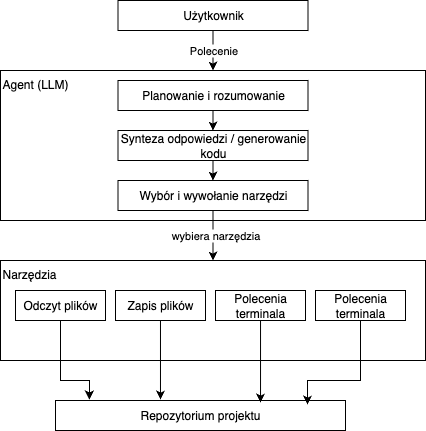
\includegraphics[width=0.8\linewidth]{img/architektura-agent.png}
    \caption{Architektura pojedynczego agenta}
    \label{fig:architektura-pojedynczego-agenta}
\end{figure}

Na rysunku \ref{fig:architektura-pojedynczego-agenta} pokazano minimalny przepływ pracy w eksperymentach dla jednego agenta. Agent otrzymuje wejście (prompt/specyfikację), następnie tworzy plan działania (kroki i artefakty), po czym iteracyjnie korzysta z narzędzi do odczytu istniejących plików i zapisu nowych zmian w repozytorium. Agent sprawdza zgodność wygenerowanego kodu z planem i wymaganiami, aktualizuje plan w razie niespójności i generuje kod.

\subsubsection*{Architektura dwuagentowa (architekt-programista)}
W tej konfiguracji wykorzystano:
\begin{itemize}
    \item \textbf{Agent Architekt} - odpowiedzialny za analizę wymagań, projektowanie struktury aplikacji i podział zadań. Używa narzędzi do odczytania specyfikacji aplikacji
    \item \textbf{Agent Programista} - implementujący kod według wytycznych architekta. Używa zestaw narzędzi do odczytywania i pisania plików jak i do wykonywania poleceń w terminalu.
\end{itemize}

\begin{figure}[!h]
    \centering 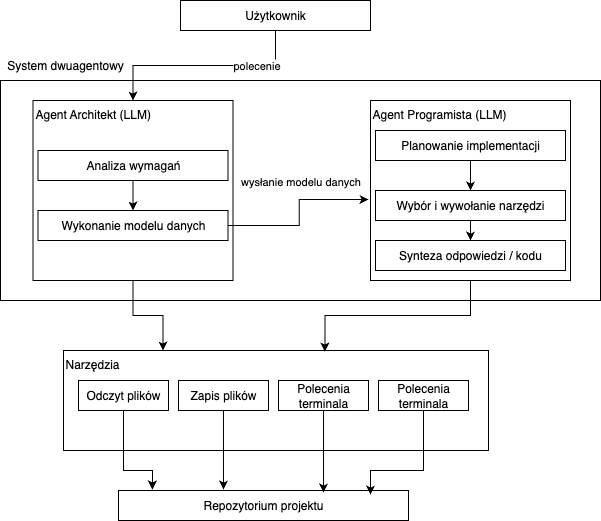
\includegraphics[width=0.9\linewidth]{img/architektura-agent-architekt.png}
    \caption{Architektura dwuagentowa: Architekt-Programista}
    \label{fig:architektura-dwuagentowa}
\end{figure}

Na rysunku \ref{fig:architektura-dwuagentowa} zilustrowano współpracę Architekta i Programisty.
Architekt rozpoczyna od analizy wejścia i tworzy artefakty koncepcyjne: proponowany model danych aplikacji. Następnie przekazuje je Programiście, który implementuje zmiany, używając Function Calling do edycji plików i wykonywania komend pomocniczych (np. formatowanie, generowanie szablonów). Komunikacja odbywa się poprzez dostęp do aktualnego repozytorium projektu, co umożliwia śledzenie kontekstu i decyzji. Proces kończy się, gdy Programista wygeneruje kod aplikacji.

\subsubsection*{Architektura wieloagentowa}
Najbardziej złożona konfiguracja obejmowała zespół wyspecjalizowanych agentów:
\begin{itemize}
    \item \textbf{Produkt Manager} - interpretacja wymagań biznesowych, utworzenie zadań i podzielenie między zespołem
    \item \textbf{Architekt systemu} - projektowanie architektury i modelu danych
    \item \textbf{Programista} - implementacja aplikacji
    \item \textbf{Recenzent kodu} - przegląd kodu i sugestie ulepszeń
\end{itemize}

\begin{figure}[!h]
    \centering 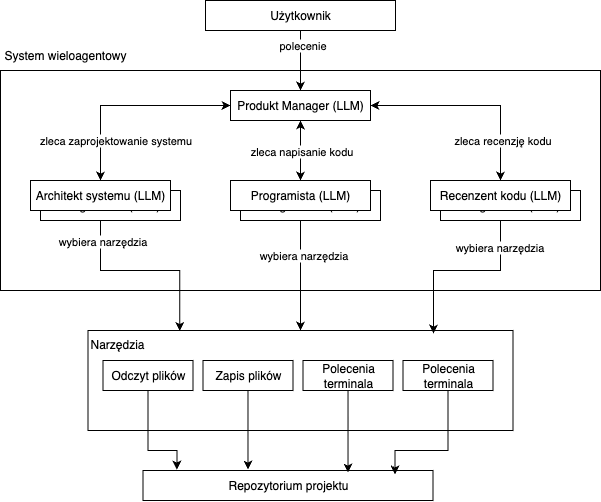
\includegraphics[width=0.9\linewidth]{img/architektura-wieloagentowa.png}
    \caption{Architektura wieloagentowa}
    \label{fig:architektura-wieloagentowa}
\end{figure}

Na rysunku \ref{fig:architektura-wieloagentowa} przedstawiono pełniejszy cykl z podziałem ról. Product Manager przyjmuje polecenie użytkownika, porządkuje wymagania i tworzy backlog zadań, Architekt definiuje model danych, Programista implementuje, a Recenzent dokonuje przeglądu zmian i zgłasza uwagi. Iteracje mają charakter bramek jakościowych: implementacja trafia do przeglądu, po akceptacji przechodzi dalej; w razie zastrzeżeń wraca do Programisty z konkretnymi poprawkami. W eksperymentach zapewniono te same wejścia, limity kroków i dostęp do narzędzi dla wszystkich konfiguracji, aby różnice w wynikach wynikały z organizacji pracy agentów, a nie z warunków testu. Zakończenie następuje po realizacji zadań oraz pozytywnej weryfikacji Recenzenta.

Koordynacja między agentami była realizowana poprzez bibliotekę OpenAI Agents SDK \cite{openai_agents_sdk_python_2025} z wykorzystaniem wzorca asynchronicznego \cite{mmazurekPythonProgramowanieAsynchroniczne} między agentami.

\clearpage
\newpage
\section{Eksperymenty}
Dla każdej z wcześniej wspomnianych konfiguracji systemu agentowego przeprowadzono eksperymenty generowania przykładowej aplikacji notatnik. W ramach danego eksperymentu przyjęto jedno z wymagań dla aplikacji biznesowej i przeprowadzono szereg testów systemu agentowego o różnych konfiguracjach. Każda konfiguracja systemu różni się między innymi liczbą, rolami agentów, poziomem autonomii agentów oraz strategią komunikacji między agentami. Celem eksperymentów było zbadanie, jak zmiany tych parametrów wpływają na ostateczny rezultat generowanej aplikacji webowej dla danych wejściowych. Dane wejściowe w tym przypadku przyjmują formę wymaganej specyfikacji dla  aplikacji notatnik. Z każdym eksperymentem poziom złożoności wymaganej aplikacji biznesowej rośnie:
\begin{itemize}
  \item pierwszy eksperyment to proste zapytanie do systemu agentowego o wygenerowanie aplikacji notatnika
  \item drugi eksperyment to zapytanie systemu agentowego o wygenerowanie aplikacji notatnika z załączoną specyfikacją w formie pliku, który zawiera wymagania kilku funkcjonalności dla aplikacji notatnika
  \item trzeci to z kolei zapytanie systemu agentowego o wygenerowanie aplikacji notatnika z załączoną zaawansowaną specyfikacją notatnika w formie pliku, która zawiera bardzo złożone i niestandardowe funkcjonalności
\end{itemize}

Każde z testów, którego wykonanie przez system agentowy wygenerowało kod oraz model danych aplikacji. Oba rezultaty danego testu zostały ocenione przez autora w skali od 1 (bardzo słabo) do 5 (bardzo dobrze) w czterech kategoriach. Kategorie opisano wraz z kryteriami oceny:
\begin{itemize}
    \item funkcjonalność - kod powinien być zgodny z wymaganiami użytkownika i wykonywać określone funkcje
    \item interfejs użytkownika - interfejs powinien być intuicyjny w użyciu
    \item estetyka - design powinien być estetycznie przyjemny i spójny
    \item brak błędów - kod powinien być wolny od błędów
\end{itemize}

Dodatkowo dla każdego eksperymentu zmierzono czas generowania aplikacji oraz liczbę użytych tokenów, co pozwala na ocenę kosztu obliczeniowego poszczególnych konfiguracji systemu agentowego.

Eksperymenty przeprowadzono w październiku 2025 roku, wykorzystując język angielski, który jest powszechnie używany w środowisku programistycznym. Wykorzystano Claude Opus 4. Taki wybór ułatwił jednolitą analizę i porównanie wyników, zapewniając spójność i wiarygodność podczas testów, a także ułatwi ewentualne dalsze porównania z innymi badaniami przeprowadzanymi w międzynarodowym środowisku programistycznym.

\subsection{Eksperyment z podstawową aplikacją}
Pierwszy eksperyment polegał na ocenie możliwości systemu agentowego w najprostszej konfiguracji zadaniowej. System otrzymał zapytanie w języku naturalnym (angielskim) o wygenerowanie aplikacji notatnika bez dodatkowej dokumentacji ani szczegółowej specyfikacji. Celem eksperymentu było sprawdzenie, jak system radzi sobie z interpretacją ogólnego polecenia oraz jakie są możliwości generacyjne w domyślnych warunkach.

W pierwszym scenariuszu wysłano ogólne polecenie utworzenia notatnika systemu opartego o jednego agenta. W drugim scenariuszu wysłano polecenie systemowi opartemu o dwóch agentów, natomiast w trzecim scenariuszu wysłano polecenie systemowi opartemu o trzech agentów.

Podczas tworzenia prostej, generycznej aplikacji notatnika systemy mogą napotkać specyficzne wyzwania. Zastosowanie podejścia wieloagentowego w takim przypadku może okazać się przerostem formy nad treścią, ponieważ dodatkowa złożoność i generowanie niepotrzebnych rozwiązań nie są uzasadnione przy tak niewielkim projekcie. W przeciwieństwie do tego, system oparty na pojedynczym agencie powinien bez problemu sprostać wymaganiom prostego notatnika.

\subsubsection*{Scenariusz 1 - podstawowy agent}
System jednego agenta był w stanie wygenerować kod aplikacji notatnika. Czas generowania aplikacji wyniósł 5 minut. Aplikacja włącza się poprawnie. Dodawanie nowych notatek, jak i usuwanie, działa bez błędów. Aplikacja posiada również funkcję edytowania notatek, która także działa. Ostatnią funkcją aplikacji jest wyszukiwanie notatek, które również działa. Interfejs użytkownika jest prosty i intuicyjny. Ogólna ocena eksperymentu pokazała, że system agentowy w najprostszej konfiguracji może być przydatny do szybkiego generowania prototypów bardzo prostych aplikacji.

\subsubsection*{Scenariusz 2 - przepływ danych w systemie architekt - programista}
Podczas tego scenariusza system wygenerował bardziej złożoną aplikację. Czas generowania aplikacji wyniósł 10 minut. Poza podstawowymi funkcjami, które wymieniono w poprzednim scenariuszu, znalazły się takie funkcje jak: organizacja notatek w folderach, oznaczanie notatek tagami, eksportowanie i importowanie notatek. W odróżnieniu od poprzedniego scenariusza, gdzie wygenerowano pojedynczy skrypt, w tym scenariuszu kod jest kompletnym projektem opartym o framework React i spełnia standardy jakości. Należy zauważyć, że aplikacja estetycznie bardzo odbiega jakością od poprzedniego scenariusza.

\subsubsection*{Scenariusz 3 - autonomiczny system wieloagentowy}
W wyniku scenariusza powstała aplikacja przypominająca scenariusz 1, z tą różnicą, że jest bardziej dopracowana, a czas jej generowania wyniósł 15 minut. Aplikacja posiada te same funkcjonalności, jednak poza nimi występują również notyfikacje o pomyślnie zapisanej lub usuniętej notatce. Interfejs użytkownika również jest dopracowany względem scenariusza 1.

\subsubsection*{Wyniki}
Wyniki wskazują, że dla prostego celu (notatnik bez szczegółowej specyfikacji) najlepszy kompromis jakości i kosztu osiąga konfiguracja z jednym agentem: najwyższa ocena funkcjonalności i stabilności (brak błędów) przy akceptowalnej estetyce i prostym, czytelnym interfejsie. Układ architekt–programista poszerza zakres rozwiązania, lecz obniża jakość interfejsu i estetyki, mimo zachowania stabilności. Należy podkreślić, że żaden scenariusz nie wygenerował błędów, które przeszkodziłyby aplikacji w funkcjonowaniu.

W konsekwencji, dla zadań o niskiej złożoności zalecane jest użycie pojedynczego agenta. Konfiguracje wieloagentowe mają uzasadnienie dopiero przy bogatszych wymaganiach wejściowych oraz jasno zdefiniowanych rolach.

\begin{table}[h!]
    \centering
    \begin{tabular}{|c|c|c|c|c|}
    \hline
    & \textbf{S1} & \textbf{S2} & \textbf{S3} \\
    \hline
    \textbf{funkcjonalność} & 4 & 5 & 4 \\
    \hline
    \textbf{interfejs użytkownika} & 4 & 3 & 5 \\
    \hline
    \textbf{estetyka} & 4 & 1 & 5 \\
    \hline
    \textbf{brak błędów} & 5 & 5 & 5 \\
    \hline
    \textbf{czas generowania} & 5 min & 10 min & 15 min \\
    \hline
    \textbf{liczba tokenów} & 12k & 28k & 45k \\
    \hline
    \end{tabular}
    \caption{Wyniki eksperymentu wygenerowania aplikacji na podstawie prostego zapytania}
    \label{table:eksperyment-proste-polecenie-utworzenia-aplikacji}
\end{table}

\subsection{Eksperyment z aplikacją na podstawie specyfikacji}
W drugim eksperymencie system agentowy otrzymał zapytanie o wygenerowanie aplikacji notatnika wraz z dołączoną podstawową specyfikacją w formie pliku tekstowego. Specyfikacja zawierała listę funkcji, które aplikacja powinna posiadać (np. dodawanie, edycja i usuwanie notatek), uproszczony model danych oraz ogólne wymagania dotyczące interfejsu użytkownika. Celem eksperymentu było sprawdzenie, w jakim stopniu system agentowy potrafi wykorzystać prostą dokumentację techniczną do wygenerowania aplikacji.

\subsubsection*{Scenariusz 1 - podstawowy agent}
Pojedynczy agent analizujący dokumentację był w stanie poprawnie wygenerować kod, który odpowiadał większości założeń ze specyfikacji. Czas generowania aplikacji wyniósł 15 minut.

\subsubsection*{Scenariusz 2 - system architekt-programista}
W tym scenariuszu jeden agent analizował wymagania, a drugi generował kod. Czas generowania aplikacji wyniósł 25 minut. Taka separacja ról pozwoliła uzyskać kod lepiej odwzorowujący specyfikację. W tym wypadku przepływ danych kilku agentów na podstawie dostarczonej podstawowej specyfikacji znacząco poprawia jakość wygenerowanej aplikacji.

Interfejs użytkownika był znacznie lepszy niż w poprzednim scenariuszu, co potwierdza pozytywny wpływ wyspecjalizowanych ról agentów na końcowy rezultat.

\subsubsection*{Scenariusz 3 - autonomiczny system wieloagentowy}
Dodanie kilku dodatkowych agentów autonomicznych odpowiedzialnych za programowanie zaowocowało bardziej kompletną aplikacją, która lepiej odpowiadała założeniom estetycznym i funkcjonalnym. Czas generowania aplikacji wyniósł 40 minut. Interfejs był bardziej dopracowany, a struktura aplikacji wyraźnie rozdzielała warstwy frontend i backend.

System agentowy z wyraźnym podziałem ról lepiej radzi sobie z przetwarzaniem wymagań i implementacją aplikacji przypominającej aplikację produkcyjną.

\subsubsection*{Wyniki}
Dostarczona specyfikacja wyraźnie poprawia jakość rezultatów względem prostego zapytania. Pojedynczy agent zapewnia wysoką stabilność i zgodność ze standardami, lecz nie domyka funkcjonalności i oferuje skromny interfejs. Układ architekt–programista poprawia jakość UI i odwzorowanie wymagań.

Najlepsze wyniki uzyskano w autonomicznym układzie wieloagentowym — pełna funkcjonalność oraz dopracowany interfejs. Przy specyfikacji o takiej szczegółowości korzyści z podziału ról i współpracy agentów przeważają koszty koordynacji. Wywnioskowano, że dla zadań opartych na podstawowej specyfikacji wieloagentowy system z jasnymi rolami jest najwydajniejszy. Gdy zasoby lub orkiestracja są ograniczone, kompromisem jest duet architekt–programista; pojedynczy agent pozostaje opcją do szybkich prototypów.

\begin{table}[h!]
    \centering
    \begin{tabular}{|c|c|c|c|c|}
    \hline
    & \textbf{S1} & \textbf{S2} & \textbf{S3} \\
    \hline
    \textbf{funkcjonalność} & 4 & 4 & 5 \\
    \hline
    \textbf{interfejs użytkownika} & 5 & 5 & 5 \\
    \hline
    \textbf{estetyka} & 3 & 4 & 5 \\
    \hline
    \textbf{brak błędów} & 5 & 5 & 5 \\
    \hline
    \textbf{czas generowania} & 15 min & 25 min & 40 min \\
    \hline
    \textbf{liczba tokenów} & 35k & 62k & 98k \\
    \hline
    \end{tabular}
    \caption{Wyniki eksperymentu aplikacji na podstawie specyfikacji}
    \label{table:eksperyment-z-aplikacja-na-podstawie-specyfikacji}
\end{table}

\subsection{Eksperyment z zaawansowaną specyfikacją aplikacji}
W trzecim eksperymencie system agentowy otrzymał zapytanie o wygenerowanie aplikacji notatnika, do którego dołączono bardziej szczegółową i zaawansowaną specyfikację techniczną w formie pliku tekstowego. Dokument ten zawierał rozszerzoną listę funkcjonalności (takich jak eksport w formacie HTML/Markdown, motywy interfejsu ciemny/jasny, widok z kalendarzem), przykładowe scenariusze użytkownika (user stories) oraz bardziej precyzyjne wytyczne związane z interfejsem użytkownika i estetyką aplikacji.

Celem tego eksperymentu było zbadanie, w jakim stopniu systemy agentowe potrafią przetworzyć złożone wymagania i wygenerować kod, który odpowiada bardziej zaawansowanej aplikacji.

\subsubsection*{Scenariusz 1 - podstawowy agent}
Pojedynczy agent nie był w stanie efektywnie poradzić sobie z całością złożonej dokumentacji. Czas generowania aplikacji wyniósł 30 minut. Wygenerowany kod obejmował jedynie podstawowe funkcje i nie uwzględniał wielu istotnych aspektów specyfikacji. Interfejs był niespójny, a struktura aplikacji nie spełniała standardów produkcyjnych. Pokazuje to ograniczenia prostych konfiguracji agentowych w kontekście bardziej wymagających zadań. Należy zaznaczyć, że agent w pierwszej próbie wygenerował aplikację z błędem, który powstrzymywał aplikację od działania. Kolejna próba rozwiązała problem, jednak z tego względu kategoria "brak błędów" otrzymała ocenę 3.

\subsubsection*{Scenariusz 2 - system architekt-programista}
W tym wariancie zastosowano podział ról: jeden agent pełnił funkcję analityczną (architekt), interpretując dokumentację, natomiast drugi – implementacyjną (programista). Czas generowania aplikacji wyniósł 1 godzinę. W rezultacie powstała aplikacja bardziej zgodna ze specyfikacją. Architekt był w stanie wyodrębnić istotne komponenty aplikacji oraz zaprojektować strukturę, co ułatwiło programiście wygenerowanie bardziej dopracowanego kodu. Interfejs był lepiej zaplanowany, choć nadal pojawiały się drobne niedociągnięcia w integracji funkcji. W tym scenariuszu pierwsza próba również zakończyła się aplikacją z błędami, dlatego wystawiono podobną ocenę w kategorii błędów jak w poprzednim scenariuszu.

\subsubsection*{Scenariusz 3 - autonomiczny system wieloagentowy}
Najbardziej zaawansowany scenariusz wykorzystał system wieloagentowy z podziałem na wyspecjalizowane role: menedżera, architekta, programistę oraz testera. Czas generowania aplikacji wyniósł 2 godziny. Agenci wykazywali wysoki poziom autonomii i komunikowali się ze sobą za pomocą pliku planu w celu negocjacji zadań i synchronizacji pracy.

Rezultatem był projekt aplikacji, który w największym stopniu odpowiadał założeniom ze specyfikacji: pełna funkcjonalność, dobrze zaprojektowana architektura, oddzielone warstwy logiki i prezentacji, a także spójny, estetyczny interfejs.

\subsubsection*{Wyniki}
Wyniki zestawione w tabeli \ref{table:eksperyment-z-zaawansowana-specyfikacja-aplikacji} przedstawiają obserwacje jakościowe z poprzednich podrozdziałów. Scenariusz z pojedynczym agentem (S1) uzyskał najniższe noty w większości kategorii, gdyż pominął zaawansowane funkcje, jak i podczas pierwszej próby zawierał błędy, które powstrzymywały go od działania. Dwóch agentów (S2) pozwoliło na znaczące zwiększenie pokrycia wymagań oraz poprawę ergonomii interfejsu, choć utrzymała się umiarkowana liczba błędów w pierwszej wygenerowanej aplikacji. Najwyższy wynik osiągnął system wieloagentowy (S3), który zrealizował pełen zakres funkcji i zachował dobrą spójność stylistyczną.

\begin{table}[h!]
    \centering
    \begin{tabular}{|c|c|c|c|c|}
    \hline
    & \textbf{S1} & \textbf{S2} & \textbf{S3} \\
    \hline
    \textbf{funkcjonalność} & 2 & 4 & 5 \\
    \hline
    \textbf{interfejs użytkownika} & 3 & 4 & 5 \\
    \hline
    \textbf{estetyka} & 5 & 4 & 5 \\
    \hline
    \textbf{brak błędów} & 3 & 3 & 5 \\
    \hline
    \textbf{czas generowania} & 30 min & 60 m & 120 m \\
    \hline
    \textbf{liczba tokenów} & 78k & 145k & 267k \\
    \hline
    \end{tabular}
    \caption{Wyniki eksperymentu aplikacji ze złożoną specyfikacją}
    \label{table:eksperyment-z-zaawansowana-specyfikacja-aplikacji}
\end{table}

\subsection{Wnioski}
Rysunek \ref{fig:wnioski-eksperymentów} syntetyzuje oceny z trzech eksperymentów. W każdym scenariuszu uśredniono wyniki wszystkich kategorii, następnie utworzono wykres zależności między scenariuszami (konfiguracjami systemu agentowego) a eksperymentami (zadane projekty do utworzenia). Rezultaty pokazują zależność pomiędzy szczegółowością dokumentacji wejściowej a konfiguracją systemu agentowego. Im bardziej precyzyjne wymagania, tym większy sens ma inwestowanie w dodatkowe role i autonomię agentów. Przy prostych poleceniach koszty koordynacji szybko przewyższają zyski.

W scenariuszach bez specyfikacji najlepiej sprawdził się pojedynczy agent, który dostarczył stabilny, kompletny prototyp przy minimalnym narzucie organizacyjnym. Dodanie kolejnych agentów przyniosło jedynie kosmetyczne ulepszenia interfejsu.

Po wprowadzeniu podstawowej specyfikacji wyraźnie zyskały konfiguracje z wyraźnym podziałem ról. Duet architekt–programista poprawił odwzorowanie wymagań i ergonomię interfejsu, a autonomiczny układ wieloagentowy domknął brakujące funkcje oraz estetykę. Wiązało się to jednak z większym nakładem na synchronizację pracy agentów.

Najbardziej złożona dokumentacja wymagała pełnego zespołu wyspecjalizowanych agentów. Tylko scenariusz wieloagentowy osiągnął pełnię funkcjonalności i zachował spójny interfejs, choć nadal wymagał dodatkowej kontroli jakości, aby ograniczyć błędy integracyjne.

Zwiększenie liczby agentów i ich specjalizacji przekłada się na wyższą jakość, ale efekty nie rosną liniowo. Każdy dodatkowy agent wymaga skuteczniejszej koordynacji. Bez niej, wzrost złożoności może prowadzić do regresji w jakości końcowego produktu. Mimo tego systemy agentowe mają realny potencjał w automatyzacji generowania aplikacji, szczególnie gdy stosuje się dobrze przemyślaną specyfikację oraz podział ról między agentami.

Analiza kosztu obliczeniowego wykazała wyraźną zależność między liczbą agentów a zużyciem tokenów. W najprostszym eksperymencie pojedynczy agent zużył 12k tokenów, podczas gdy system wieloagentowy wymagał 45k tokenów (prawie 4-krotny wzrost). W eksperymencie ze złożoną specyfikacją różnica była jeszcze bardziej wyraźna: 78k tokenów dla pojedynczego agenta wobec 267k dla systemu wieloagentowego (ponad 3-krotny wzrost). Wzrost zużycia tokenów wynika z komunikacji między agentami, wielokrotnego przetwarzania kontekstu oraz mechanizmów koordynacji. Należy zatem rozważyć kompromis między jakością rozwiązania a kosztem obliczeniowym, szczególnie w kontekście komercyjnego wykorzystania systemów agentowych.

Systemy agentowe są więc użyteczne zarówno do szybkiego prototypowania, jak i do tworzenia bardziej złożonych aplikacji, pod warunkiem dobrania architektury do jakości specyfikacji oraz wyposażenia procesu w mechanizmy koordynacji (np. współdzieloną pamięć, inspekcje wyników). Bez nich wzrost liczby agentów nie przekłada się wprost na wyższą jakość rozwiązania.

\begin{figure}[!h]
    \centering 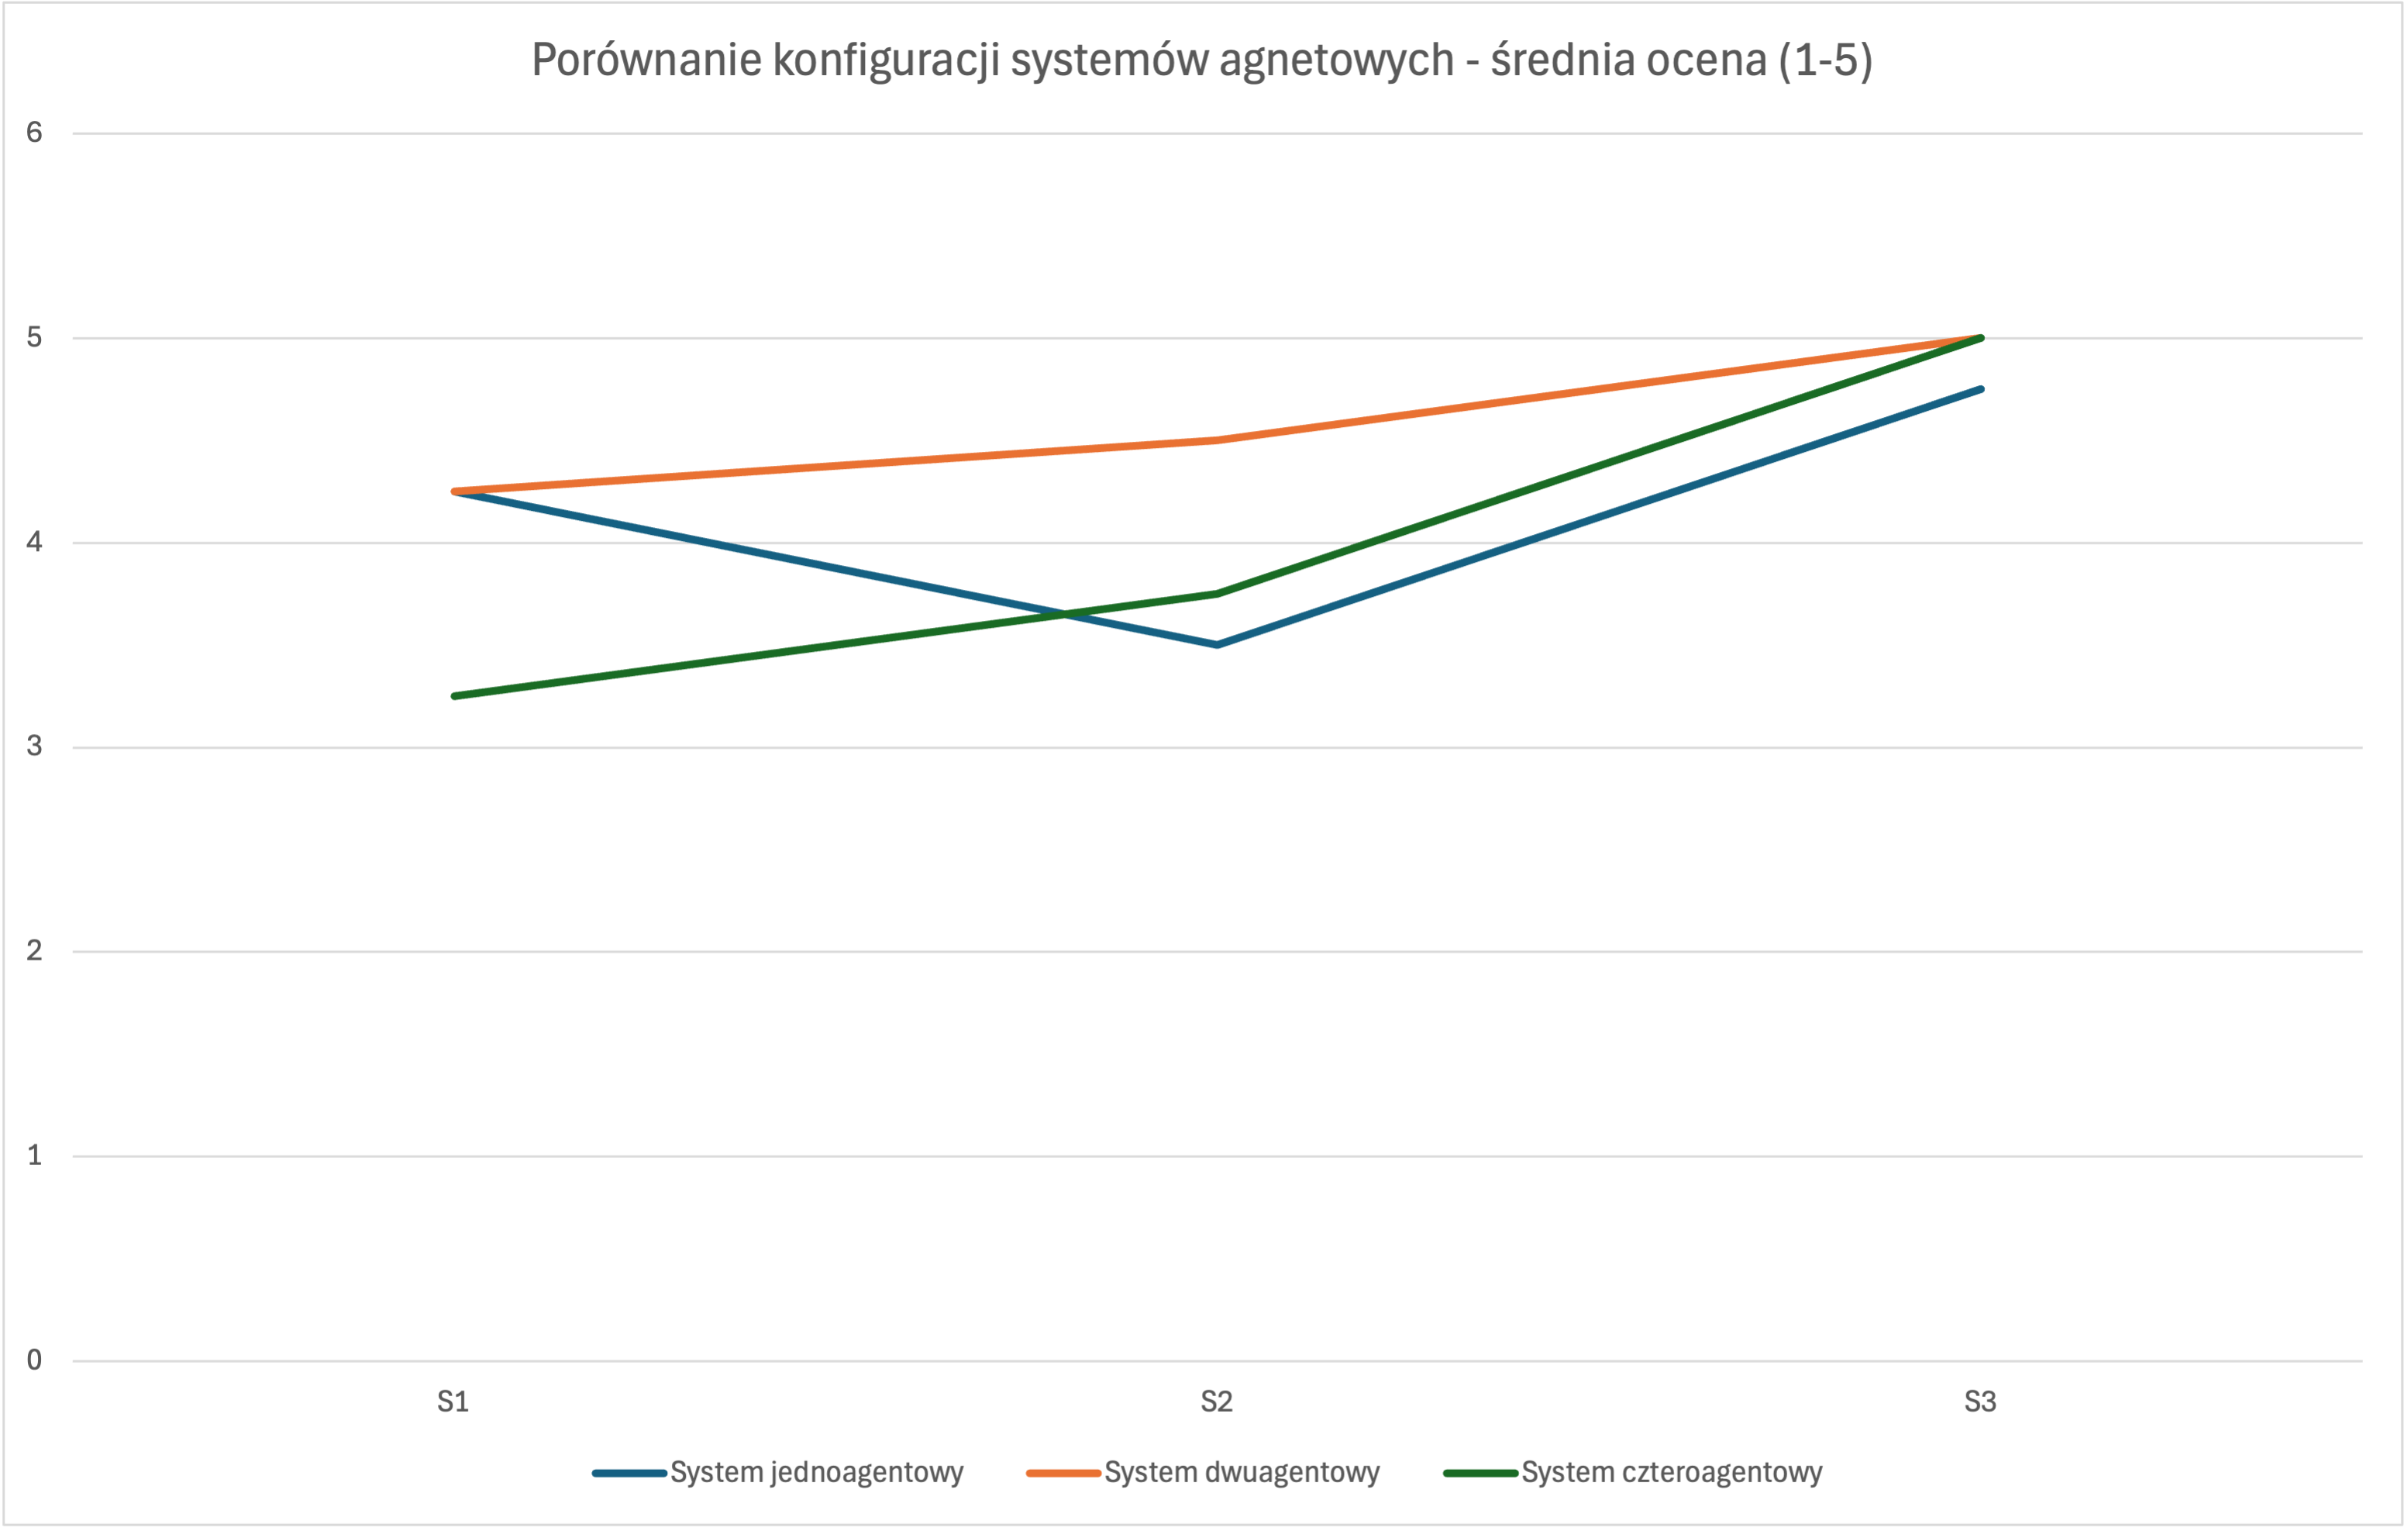
\includegraphics[width=0.9\linewidth]{img/wnioski.png}
    \caption{Uśrednione wyniki scenariuszy dla poszczególnych eksperymentów, inaczej konfiguracji systemu agentowego}
    \label{fig:wnioski-eksperymentów}
\end{figure}

\clearpage
\raggedbottom
\newpage
\section{Implementacja aplikacji biznesowej przy użyciu systemu agentowego}
Niniejszy rozdział dokumentuje wdrożenie portalu sieciowego do zarządzania serwisem samochodowym. Implementacja odpowiada trzeciemu scenariuszowi eksperymentów zaprezentowanemu na rysunku \ref{fig:architektura-wieloagentowa}, w którym konfiguracja wieloagentowa (Manager, Architekt, Programista, Recenzent) zasilana modelem Claude Opus 4 uzyskała najwyższe noty za kompletność oraz jakość. Celem iteracji było przejście pełnego cyklu wytwórczego: od planu technicznego, przez implementację, integrację z systemami zewnętrznymi i testy, po przygotowanie artefaktów wdrożeniowych.

Jako przypadek użycia systemu agentowego wybrano aplikację webową o nazwie AutoServe przeznaczoną dla właścicieli serwisów samochodowych, którzy chcą cyfrowo zarządzać swoim biznesem. Decyzja miała podkreślić zdolność LLM do generowania aplikacji spoza typowych repozytoriów kodu, w których modele były szeroko trenowane. Modele językowe bardzo dobrze radzą sobie z popularnymi aplikacjami, takimi jak notatniki czy listy zadań, ponieważ w repozytoriach otwartego źródła występuje wiele kompletnych implementacji tego typu systemów. Dla portali dedykowanych warsztatom samochodowym liczba dostępnych przykładów jest niewielka, co zwiększa wartość demonstracji.

\subsection{Obserwacja pracy systemu wieloagentowego}
Prace rozpoczęto od opracowania szczegółowej specyfikacji aplikacji do wygenerowania (załącznik), obejmującej scenariusze pracy serwisu oraz oczekiwane moduły biznesowe. Przekazano agentom wyłącznie ten artefakt, aby system samodzielnie podjął decyzje dotyczące technologii, struktury projektu oraz zakresu pierwszej inkrementacji. Agent Architekt przeanalizował dokument wymagań aplikacji (specification.md) i określił zakres MVP (Minimum Viable Product), czyli minimalnej wersji produktu. Agent następnie opracował plan implementacji, podzielony na 5 sprintów, grupujących zadania według funkcjonalności aplikacji. W ramach planowania agent wybrał następujący stos technologiczny: React 18 z TypeScript, Vite jako bundler, Zustand do zarządzania stanem aplikacji, Dexie.js jako warstwę abstrakcji nad IndexedDB, Tailwind CSS w warstwie prezentacji oraz shadcn/ui jako bibliotekę komponentów interfejsu użytkownika.

Agent Architekt, bazując na autonomicznie dobranym stosie technologicznym, przygotował szczegółową dokumentację techniczną (ARCHITECTURE.md). Agent zdecydował o architekturze local-first, w której wszystkie dane są przechowywane lokalnie w przeglądarce użytkownika za pomocą IndexedDB, bez zależności od backendu. Model danych obejmuje trzy główne encje: \texttt{customers} (klienci serwisu z danymi kontaktowymi), \texttt{vehicles} (pojazdy przypisane do klientów z danymi identyfikacyjnymi, jak VIN i numer rejestracyjny) oraz \texttt{work\_orders} (zlecenia serwisowe ze statusem, pozycjami robocizny i części oraz obliczeniami kosztów).

W następnym kroku Agent Architekt zlecił kontynuację nad projektem Agentowi Programiście, który przeprowadził implementację według planu podzielonego na 5 sprintów. Każdy cykl obejmował plan prac, modyfikacje kodu oraz lokalną weryfikację. Najważniejsze kroki przedstawiono poniżej:
\begin{enumerate}
    \item \textbf{Sprint 1: Fundament} -- wygenerowanie szkieletu projektu Vite z React i TypeScript, konfiguracja TypeScript (\texttt{tsconfig.json}, \texttt{tsconfig.app.json}), Tailwind CSS oraz instalacja i konfiguracja biblioteki komponentów shadcn/ui. Utworzono podstawową strukturę routingu z wykorzystaniem React Router oraz komponenty layoutu (Header, Navigation, MainLayout).
    \item \textbf{Sprint 2: Warstwa danych} -- implementacja schematu bazy danych w Dexie.js z trzema tabelami (\texttt{customers}, \texttt{vehicles}, \texttt{workOrders}) oraz odpowiednimi indeksami. Utworzono definicje typów TypeScript dla encji domenowych oraz zaimplementowano trzy store'y Zustand (\texttt{customerStore}, \texttt{vehicleStore}, \texttt{workOrderStore}) z mechanizmem zapisywania danych do IndexedDB i optymistycznymi aktualizacjami.
    \item \textbf{Sprint 3: Zarządzanie klientami} -- utworzenie strony listy klientów (\texttt{Customers.tsx}) z funkcją wyszukiwania i filtrowania, formularza klienta (\texttt{CustomerForm.tsx}) z walidacją Zod, widoku szczegółów klienta (\texttt{CustomerDetail.tsx}) z historią serwisową oraz modułu zarządzania pojazdami (\texttt{VehicleForm.tsx}).
    \item \textbf{Sprint 4: Zarządzanie zleceniami} -- implementacja strony listy zleceń serwisowych (\texttt{WorkOrders.tsx}) z filtrowaniem po statusie, formularza tworzenia zlecenia z dynamicznym dodawaniem pozycji kosztów, widoku szczegółów zlecenia z możliwością zmiany statusu oraz generowania wydruku faktury (\texttt{WorkOrderPrint.tsx}).
    \item \textbf{Sprint 5: Dashboard i finalizacja} -- budowa pulpitu głównego (\texttt{Dashboard.tsx}) z kluczowymi metrykami (liczba aktywnych zleceń, przychody, alerty), implementacja strony ustawień (\texttt{Settings.tsx}) z funkcjami eksportu i importu danych w formacie JSON, oraz dopracowanie interfejsu użytkownika zgodnie ze specyfikacją kolorystyczną (\#0C5EAF jako kolor główny, \#F2F5F9 dla tła).
\end{enumerate}

\subsection{Operacje agenta Recenzent}
Agent Recenzent weryfikował każdą partię zmian pod kątem jakości kodu, zgodności z wymaganiami oraz potencjalnych błędów. Ze względu na architekturę local-first aplikacji, nie wystąpiły problemy związane z synchronizacją z backendem czy uprawnieniami użytkowników -- aplikacja działa w trybie jednoużytkownikowym bez warstwy serwerowej. Validator skupił się na walidacji poprawności logiki biznesowej, obsługi błędów IndexedDB oraz spójności interfejsu użytkownika. Finałowy raport obejmował analizę struktury projektu oraz pokrycie testów.

Warstwa jakości opierała się na frameworku testowym Vitest. Przygotowano testy jednostkowe obejmujące logikę store'ów Zustand (operacje CRUD na encjach, kalkulację sum zleceń), funkcje pomocnicze w \texttt{src/lib/utils.ts} oraz walidację schematów Zod. Testy komponentów z wykorzystaniem React Testing Library weryfikowały poprawność renderowania formularzy, interakcje użytkownika oraz warunkowe wyświetlanie elementów UI. Skonfigurowano również ESLint z presetami dla React i TypeScript oraz Prettier dla zapewnienia spójnego formatowania kodu. Ze względu na ograniczenia czasowe MVP, nie zaimplementowano testów end-to-end, co zostało odnotowane jako obszar do rozwoju w kolejnych iteracjach.

\subsection{Interfejs użytkownika aplikacji}
Wygenerowana aplikacja charakteryzuje się nowoczesnym i przejrzystym interfejsem użytkownika, zgodnym z dostarczoną specyfikacją. Poniżej zaprezentowano zrzuty ekranu kluczowych widoków aplikacji.

Rysunek \ref{fig:screenshot-dashboard} przedstawia pulpit główny aplikacji. Jest to pierwszy ekran, który widzi użytkownik po uruchomieniu aplikacji. Zawiera on kluczowe wskaźniki wydajności (KPI), takie jak liczba otwartych zleceń, suma przychodów z ostatnich 30 dni oraz skróty do najczęściej używanych funkcji, takich jak dodawanie nowego klienta czy zlecenia. Projekt interfejsu jest minimalistyczny, z wyraźnym naciskiem na czytelność danych.

\begin{figure}[h!]
    \centering
    \includegraphics[width=\textwidth]{img/dashboard.png}
    \caption{Pulpit główny aplikacji AutoServe, prezentujący kluczowe metryki i skróty do najważniejszych funkcji.}
    \label{fig:screenshot-dashboard}
\end{figure}

Na rysunku \ref{fig:screenshot-customers} widoczny jest widok listy klientów. Umożliwia on przeglądanie wszystkich zapisanych klientów wraz z ich podstawowymi danymi kontaktowymi. Użytkownik ma możliwość wyszukiwania klientów po imieniu, nazwisku lub numerze telefonu. Z tego poziomu można również przejść do edycji danych klienta lub dodać nowego klienta do bazy, co jest kluczową funkcją w codziennej pracy serwisu.

\begin{figure}[h!]
    \centering
    \includegraphics[width=\textwidth]{img/customers-list.png}
    \caption{Widok listy klientów z funkcją wyszukiwania i możliwością dodania nowego klienta.}
    \label{fig:screenshot-customers}
\end{figure}

Rysunek \ref{fig:screenshot-work-order} prezentuje formularz tworzenia nowego zlecenia serwisowego. Jest to jeden z bardziej złożonych interfejsów w aplikacji. Formularz pozwala na przypisanie zlecenia do istniejącego klienta i pojazdu, a także na dynamiczne dodawanie pozycji serwisowych, zarówno usług, jak i części. System automatycznie oblicza sumę kosztów, co minimalizuje ryzyko pomyłek. Interfejs został zaprojektowany tak, aby prowadzić użytkownika krok po kroku przez proces tworzenia zlecenia.

\begin{figure}[h!]
    \centering
    \includegraphics[width=\textwidth]{img/work-order-form.png}
    \caption{Formularz tworzenia nowego zlecenia serwisowego z dynamicznie dodawanymi pozycjami.}
    \label{fig:screenshot-work-order}
\end{figure}

\clearpage

\subsection{Ocena efektywności procesu}
Proces implementacji przeprowadzono w ramach sesji z systemem wieloagentowym, która trwała około dwóch godzin. Całość prac obejmowała fazę planowania (agent Architekt), implementację (agent Builder) oraz walidację (agent Validator). System wygenerował kompletną aplikację MVP spełniającą część wymagań funkcjonalnych określonych w specyfikacji. Dzięki architekturze local-first, aplikacja mogła być uruchomiona bez dodatkowych konfiguracji żadnych zewnętrznych usług czy kluczy API, a wszystkie dane są przechowywane lokalnie w przeglądarce użytkownika.

Projekt finalnie liczy 39 plików źródłowych w języku TypeScript oraz 7 plików konfiguracyjnych. Struktura katalogów obejmuje: 14 komponentów UI w katalogu \texttt{src/components}, 7 stron aplikacji w katalogu \texttt{src/pages}, warstwę bazodanową Dexie.js w \texttt{src/db} oraz funkcje pomocnicze w \texttt{src/lib}. Aplikacja wykorzystuje 29 zależności produkcyjnych (m.in. React, Zustand, Dexie, Zod, date-fns, lucide-react) oraz 21 zależności deweloperskich (m.in. Vite, TypeScript, ESLint, Vitest, Testing Library).

\begin{figure}[!h]
    \centering \includegraphics[width=0.8\linewidth]{img/functionalities-pie-chart.png}
    \caption{Podział funkcjonalności na zaimplementowane i niezaimplementowane}
    \label{fig:wykres-kolowy-implementacji}
\end{figure}

Z 63 funkcjonalności zaplanowanych w specyfikacji, system agentowy zaimplementował 29 (46\%), pozostawiając 34 (54\%) jak pokazano na rysunku \ref{fig:wykres-kolowy-implementacji}. Interfejs użytkownika oraz estetyka uzyskały notę 5, natomiast kategoria funkcjonalność otrzymała 3, a brak błędów 4 ze względu na błąd w konfiguracji stylizacji aplikacji, którą recenzent musiał samodzielnie poprawić w pliku \texttt{tailwind.config.js}.

\subsection{Wnioski}
Implementacja AutoServe pokazała, że wieloagentowa konfiguracja sprawdza się przy złożonych aplikacjach biznesowych, o ile towarzyszy jej precyzyjny dokument wymagań oraz jasna definicja zakresu MVP oraz ścisła kontrola jakości. Największą wartość wniosła szczegółowa dokumentacja architektoniczna (ARCHITECTURE.md) przygotowana przez agenta Architekt, która stanowiła punkt odniesienia dla agenta Programisty podczas implementacji. Jasno zdefiniowane wzorce architektoniczne (local-first, optymistyczne aktualizacje, persystencja z Zustand) pozwoliły uniknąć problemów projektowych na etapie kodowania.

System wieloagentowy wykazał się szczególną skutecznością w wyborze odpowiedniego stosu technologicznego - decyzja o architekturze local-first była trafna dla przypadku użycia (brak potrzeby wdrażania oprogramowania na serwerze). Wybór Dexie.js jako warstwy abstrakcji nad IndexedDB oraz Zustand jako lekkiego state managera okazał się optymalny dla aplikacji MVP, pozwalając na bezproblemową implementację. W tabeli \ref{table:wyniki-wygenerowanej-aplikacji-biznesowej} przedstawiono wyniki wygenerowanej aplikacji analogicznie do poprzedniego eksperymentu.

\begin{table}[h!]
    \centering
    \begin{tabular}{|c|c|c|c|c|}
    \hline
    & \textbf{Ocena} \\
    \hline
    \textbf{funkcjonalność} & 3 \\
    \hline
    \textbf{interfejs użytkownika} & 5 \\
    \hline
    \textbf{estetyka} & 5 \\
    \hline
    \textbf{brak błędów} & 4 \\
    \hline
    \textbf{czas generowania} & 120 m \\
    \hline
    \end{tabular}
    \caption{Wyniki wygenerowanej aplikacji biznesowej}
    \label{table:wyniki-wygenerowanej-aplikacji-biznesowej}
\end{table}

Na kolejne iteracje eksperymentu rekomenduje się rozszerzenie pokrycia testowego o testy end-to-end z wykorzystaniem Playwright lub Cypress, które zweryfikują pełne scenariusze użytkownika (od utworzenia klienta, przez rejestrację pojazdu, po wygenerowanie zlecenia i faktury) tak, aby zbadać, czy system agentowy zaimplementowałby zaawansowane funkcje zaplanowane w dokumentacji architektonicznej, takie jak: wsparcie dla skrótów klawiszowych oraz widok kalendarza z nadchodzącymi wizytami klientów. Doświadczenie z AutoServe potwierdza, że system agentowy może samodzielnie wygenerować aplikację biznesową o jakości MVP, jeśli otrzyma dobrze zdefiniowane wymagania funkcjonalne i niefunkcjonalne.

\clearpage
\section{Podsumowanie}

Praca miała na celu empiryczną ocenę wpływu agentów AI opartych na dużych modelach językowych (LLM) na proces tworzenia oprogramowania, ze szczególnym uwzględnieniem różnych konfiguracji systemów agentowych. W ramach badań zrealizowano trzy główne eksperymenty oraz rzeczywistą implementację aplikacji biznesowej, aby zweryfikować skuteczność systemów agentowych w zróżnicowanych scenariuszach wytwarzania oprogramowania.

W części teoretycznej przedstawiono fundamenty działania modeli językowych, w tym architekturę Transformer, mechanizmy tokenizacji i osadzania wektorowego oraz kluczowe ograniczenia współczesnych LLM. Szczególną uwagę poświęcono koncepcji agentów AI jako rozszerzeń modeli językowych wyposażonych w narzędzia, pamięć i zdolności rozumowania. Przeanalizowano również systemy wieloagentowe (MAS), w których wyspecjalizowani agenci współpracują w ramach zdefiniowanych ról, co pozwala na dekompozycję złożonych zadań programistycznych.

W części eksperymentalnej przeprowadzono serię kontrolowanych testów z trzema konfiguracjami systemu agentowego: pojedynczy agent uniwersalny, układ dwuagentowy (architekt-programista) oraz autonomiczny system wieloagentowy (manager-architekt-programista-recenzent). Każda konfiguracja została przetestowana w trzech scenariuszach o rosnącej złożoności: proste zapytanie bez dokumentacji, zapytanie z podstawową specyfikacją oraz zapytanie z zaawansowaną dokumentacją techniczną. Wygenerowane aplikacje oceniano w czterech kategoriach: funkcjonalność, interfejs użytkownika, estetyka oraz brak błędów.

Wyniki eksperymentów ujawniły wyraźną zależność między szczegółowością dokumentacji wejściowej a optymalną konfiguracją systemu agentowego. Dla prostych zadań bez specyfikacji pojedynczy agent osiągał najlepsze rezultaty przy minimalnym narzucie organizacyjnym. Wprowadzenie podstawowej specyfikacji sprawiło, że układy dwu- i wieloagentowe znacząco poprawiły jakość odwzorowania wymagań oraz estetykę interfejsu. W przypadku zaawansowanej dokumentacji technicznej wyłącznie system wieloagentowy był w stanie zrealizować pełen zakres funkcjonalności przy zachowaniu spójności architektonicznej i stabilności działania.

Praktyczną walidację wniosków stanowiła implementacja aplikacji biznesowej AutoServe - portalu do zarządzania serwisem samochodowym. System wieloagentowy autonomicznie opracował architekturę local-first opartą o React, TypeScript i IndexedDB, przeprowadził implementację w pięciu sprintach oraz zapewnił warstwę testów jednostkowych. Aplikacja finalna składała się z 39 plików źródłowych i spełniała większość wymagań funkcjonalnych MVP. Proces wytwórczy trwał około godziny i wykazał zdolność systemu do samodzielnego doboru stosu technologicznego oraz realizacji złożonych scenariuszy biznesowych.

Najważniejsze wnioski z badań to: systemy agentowe wykazują realny potencjał w automatyzacji wytwarzania oprogramowania, szczególnie przy dobrze zdefiniowanych wymaganiach; efektywność rozwiązania nie rośnie liniowo ze wzrostem liczby agentów - wymaga to skutecznych mechanizmów koordynacji i kontroli jakości; pojedynczy agent pozostaje optymalny dla prototypowania prostych aplikacji, natomiast konfiguracje wieloagentowe znajdują uzasadnienie w projektach o wysokiej złożoności funkcjonalnej; jakość dokumentacji wejściowej bezpośrednio determinuje skuteczność systemu agentowego - im bardziej precyzyjne wymagania, tym lepsze odwzorowanie w kodzie.

Przeprowadzone badania potwierdzają tezę, że agenty AI stanowią wartościowe narzędzie wspierające proces wytwarzania oprogramowania. Jednakże ich skuteczność jest warunkowa i zależy od dopasowania konfiguracji systemu do specyfiki zadania oraz jakości dokumentacji wymagań. Dalsze badania powinny skupić się na mechanizmach koordynacji w większych zespołach agentowych, metodach automatycznej walidacji jakości generowanego kodu oraz długoterminowych kosztach utrzymania aplikacji wytworzonych przez systemy agentowe.


\newpage

%--------------------------------------------
% Literatura
%--------------------------------------------
\cleardoublepage
\printbibliography

%--------------------------------------------
% Spisy (opcjonalne)
%--------------------------------------------
\newpage
\pagestyle{plain}

% Wykaz symboli i skrótów.
% Pamiętaj, żeby posortować symbole alfabetycznie
% we własnym zakresie. Ponieważ mało kto używa takiego wykazu,
% uznałem, że robienie automatycznie sortowanej listy
% na poziomie LaTeXa to za duży overkill.
% Makro \acronymlist generuje właściwy tytuł sekcji,
% w zależności od języka.
% Makro \acronym dodaje skrót/symbol do listy,
% zapewniając podstawowe formatowanie.
% //AB
\vspace{0.8cm}
\acronymlist
\acronym{EE}{Wydział Elektryczny}
\acronym{PW}{Politechnika Warszawska}
\acronym{WEIRD}{ang. \emph{Western, Educated, Industrialized, Rich and Democratic}}

\listofappendicestoc  % Spis załączników

% Załączniki
\newpage
\appendix{Nazwa załącznika 1}

\newpage
\appendix{Nazwa załącznika 2}

% Używając powyższych spisów jako szablonu,
% możesz tu dodać swój własny wykaz bądź listę,
% np. spis algorytmów.

\end{document}
